\section{Deviations of Random Matrices on Sets}
The main question in this chapter is: How does an $m \times n$ matrix act on a general set $t \subset 
\mathbb{R}^n$? 



% ----------9.1----------
\subsection{Matrix Deviation Inequality}
Take an $m \times n$ random matrix $X$ with independent, isotropic, and subgaussian rows. The concentration of 
the norm (\cref{thm:3.1.1}) tells us that for any fixed vector $x \in \mathbb{R}^n$, the approximation 
\[ \lVert Ax \rVert_{2} \approx \sqrt{m}\lVert x \rVert_{2} \]
holds with high probability.

Let's ask something more general: Is it true that with high probability, the equation above holds 
\textit{simultaneously} for many vectors $x \in \mathbb{R}^n$? To quantify how many, pick some bounded set 
$T \subset \mathbb{R}^n$ and ask if the approximation holds simultaneously for all $x \in T$. It turns out that 
the maximal error is about $\gamma(T)$, the Gaussian complexity of $T$.

\begin{theorem}[Matrix deviation inequality]
\label{thm:9.1.1}
Let $A$ be an $m \times n$ random matrix with independent, isotropic and subgaussian rows $A_i$. Then for any 
subset $T \subset \mathbb{R}^n$, 
\[ \mathbb{E}\left[ \sup_{x \in T}\left| \lVert Ax \rVert_{2} - \sqrt{m}\lVert x \rVert_{2} \right| \right] 
\leq CK^2 \gamma(T), \]
where $\gamma(T)$ is the Gaussian complexity from Section 7.5.3, defined as 
\[ \gamma(T) = \mathbb{E}\left[ \sup_{x \in T}|\left\langle g, x \right\rangle| \right], \ g \sim N(0, I_n), \]
and $K = \max_{i} \lVert A_i \rVert_{\psi_2}$.
\end{theorem}

The plan is to deduce this from Talagrand's comparison inequality (\cref{cor:8.5.8}). To do that, we just have 
to check the random process 
\[ Z_x := \lVert Ax \rVert_{2} - \sqrt{m}\lVert x \rVert_{2} \]
indexed by vectors $x \in \mathbb{R}^n$ has subgaussian increments. Here is the claim:

\begin{theorem}[Subgaussian increments]
\label{thm:9.1.2}
Let $A$ be an $m \times n$ random matrix with independent, isotropic and subgaussian rows $A_i$. Then the random 
process $Z_x$ defined above has subgaussian increments: 
\[ \lVert Z_x - Z_y \rVert_{\psi_2} \leq CK^2 \lVert x - y \rVert_{2} \text{ for all } x, y \in \mathbb{R}^n, \]
here $K = \max_{i} \lVert A_i \rVert_{\psi_2}$.
\end{theorem}

Once we have proved this theorem, we plug it into Talagrand's comparison inequality (Exercise 8.37 (a)) and get 
\[ \mathbb{E}\left[ \sup_{x \in T} |Z_x| \right] \leq CK^2 \gamma(T) \]
which directly gives \cref{thm:9.1.1}. So, all we have to do is prove \cref{thm:9.1.2} - and it is in fact 
easier since it's for fixed $x$ and $y$.

\begin{proof}[Proof of \cref{thm:9.1.2}]
This argument will be a bit longer than usual, so we'll (hopefully) make it easier by starting with simpler 
cases and building up from there.

\textbf{Step 1: Unit vector $x$ and zero vector $y$.} If $\lVert x \rVert_{2} = 1$ and $y = 0$, the inequality 
in the theorem statement becomes 
\[ \left\lVert \lVert Ax \rVert_{2} - \sqrt{m} \right\rVert_{\psi_2} \leq CK^2. \]
The random vector $Ax \in \mathbb{R}^m$ has independent, subgaussian coordinates $\left\langle A_i, x
\right\rangle$, which satisfy 
\[ \mathbb{E}\left[ \left\langle A_i, x \right\rangle^2 \right] = 1 \] 
by isotropy. So, the equation above follows from the concentration of the norm (\cref{thm:3.1.1}).

\textbf{Step 2: Unit vectors $x, y$ and the squared process.} Assume now that 
\[ \lVert x \rVert_{2} = \lVert y \rVert_{2} = 1. \]
In this case, the inequality in the theorem statement becomes 
\[ \left\lVert \lVert Ax \rVert_{2} - \lVert Ay \rVert_{2} \right\rVert_{\psi_2} \leq 
CK^2 \lVert x - y \rVert_{2}. \quad (*) \]
Since the \textit{squared} $\ell^2$ norm would be simpler to work with (no square roots), let's prove a version 
of the equation above with squared norms. Here's a good guess to what it should look like: with high probability,
\begin{align*}
	\lVert Ax \rVert_{2}^2 - \lVert Ay \rVert_{2}^2 
	&= (\lVert Ax \rVert_{2} + \lVert Ay \rVert_{2}) \cdot (\lVert Ax \rVert_{2} - \lVert Ay \rVert_{2}) \\
	&\lesssim \sqrt{m} \cdot \lVert x - y \rVert_{2}.
\end{align*}
This seems reasonable because $\lVert Ax \rVert_{2}$ and $\lVert Ay \rVert_{2}$ are roughly $\sqrt{m}$ by step 
1, and hence we expect $(*)$ to hold.

Let's go ahead and prove this. Expand the matrix-vector product:
\[ \lVert Ax \rVert_{2}^2 - \lVert Ay \rVert_{2}^2 
= \sum_{i = 1}^{m} (\left\langle A_i, x \right\rangle^2 - \left\langle A_i, y \right\rangle^2) 
= \sum_{i = 1}^{m} \left\langle A_i, x + y \right\rangle \left\langle A_i, x - y \right\rangle, \]
then dividing both sides by $\lVert x - y \rVert_{2}$, getting 
\[ \Delta := \frac{\lVert Ax \rVert_{2}^2 - \lVert Ay \rVert_{2}^2}{\lVert x - y \rVert_{2}^2} 
= \sum_{i = 1}^{m} \left\langle A_i, u \right\rangle \left\langle A_i, v \right\rangle, \]
where 
\[ u := x + y \text{ and } v := \frac{x - y}{\lVert x - y \rVert_{2}}. \]
Our goal is to show that $|\Delta| \lesssim \sqrt{m}$ with high probability.

What do we see in $\Delta$? A sum of \textit{independent} random variables $\left\langle A_i, u \right\rangle 
\left\langle A_i, v \right\rangle$! They are mean-zero, because by construction we have 
\[ \left\langle A_i, u \right\rangle \left\langle A_i, v \right\rangle = 
\frac{\left\langle A_i, x \right\rangle^2 - \left\langle A_i, y \right\rangle^2}{\lVert x - y \rVert_{2}}, \]
and by isotropy, 
\[ \mathbb{E}\left[ \left\langle A_i, x \right\rangle^2 - \left\langle A_i, y \right\rangle^2 \right] 
= 1 - 1 = 0. \]
Moreover, these are \textit{subexponential}. \cref{lem:2.8.6} and the subgaussian assumption on $A_i$ give 
\begin{align*}
	\lVert \left\langle A_i, u \right\rangle \left\langle A_i, v \right\rangle \rVert_{\psi_1} 
	&\leq \lVert \left\langle A_i, u \right\rangle \rVert_{\psi_2} \cdot 
	\lVert \left\langle A_i, v \right\rangle \rVert_{\psi_2} \\
	&\leq K \lVert u \rVert_{2} \cdot K \lVert v \rVert_{2} \\
	&\leq 2K^2
\end{align*}
where in the last step, we used that $\lVert u \rVert_{2} \leq \lVert x \rVert_{2} + \lVert y \rVert_{2} \leq 2$ 
and $\lVert v \rVert_{2} = 1$. So we can apply Bernstein's inequality (\cref{thm:2.9.1}) and get 
\[ P(|\Delta| \geq t \sqrt{m}) \leq 2 \exp{\left[ -c \min_{}\left( \frac{t^2}{K^4}, \frac{t \sqrt{m}}{K^2} 
\right) \right]} \leq 2 \exp{\left( -\frac{c_1 t^2}{K^4} \right)} \]
for any $0 \leq t \leq \sqrt{m}$.

\textbf{Step 3: Unit vector $x, y$ and the original process.} Now let's get rid of the squares and prove the 
original inequality $(*)$ for all unit vectors $x$ and $y$.

Using the definition of the subgaussian norm (\cref{prop:2.6.6} (i) and \cref{rmk:2.6.3}), $(*)$ becomes 
\[ p(s) := P \left( \frac{|\lVert Ax \rVert_{2} - \lVert Ay \rVert_{2}|}{\lVert x - y \rVert_{2}^2} \right) 
\leq 4 \exp{\left( -\frac{cs^2}{K^2} \right)} \text{ for all } s > 0. \]
(Here the constant 4 instead of 2 will give us a little more room to maneuver.)

Now we have two cases:
\textit{Case 1:} $s \leq 2 \sqrt{m}$. Let's use the result from step 2. To use it, multiply both sides of the 
inequality that defines $p(s)$ by $\lVert Ax \rVert_{2} + \lVert Ay \rVert_{2}$, and recall the definition of 
$\Delta$ to get 
\[ p(s) = P(|\Delta| \geq s(\lVert Ax \rVert_{2} + \lVert Ay \rVert_{2})) 
\leq P(|\Delta| \geq s \lVert Ax \rVert_{2}). \]
We know from step 2 that $\lVert Ax \rVert_{2} \approx \sqrt{m}$ with high probability. So it makes sense to 
consider two cases: THe likely case where $\lVert Ax \rVert_{2} \geq \sqrt{m}/2$ and thus $|\Delta| \geq 
s \sqrt{m}/2$, and the unlikely case where $\lVert Ax \rVert_{2} < \sqrt{m}/2$ (and we deop the clause about 
$\Delta$, only increasing the probability). This leads to 
\[ p(s) \leq P \left( |\Delta| \geq \frac{s \sqrt{m}}{2} \right) + P \left( \lVert Ax \rVert_{2} 
< \frac{\sqrt{m}}{2} \right) = p_1(s) + p_2(s). \]
The result from Step 2 handles the likely case:
\[ p_1(s) \leq 2 \exp{\left( -\frac{cs^2}{K^4} \right)}, \]
while the result of Step 1 together with the triangle inequality handle the unlikely case: 
\[ p_2(s) \leq P \left( |\lVert Ax \rVert_{2} - \sqrt{m}| > \frac{\sqrt{m}}{2} \right) 
\leq 2 \exp{\left( -\frac{cs^2}{K^4} \right)}.\]
Adding up the two, we get the desired bound:
\[ p(s) \leq 4 \exp{\left( -\frac{cs^2}{K^4} \right)}. \]

\textit{Case 2:} $s > 2 \sqrt{m}$. By the triangle inequality, $|\lVert Ax \rVert_{2} - \lVert Ay \rVert_{2}| 
\leq \lVert A(x - y) \rVert_{2}$, so 
\begin{align*}
	p(s) \leq P(\lVert Au \rVert_{2} \geq s) \quad (u = \frac{x - y}{\lVert x - y \rVert_{2}} 
	\text{ as before}) \\
	&\leq P(\lVert Au \rVert_{2} - \sqrt{m} \geq s/2) \quad (\text{Since } s > 2 \sqrt{m}) \\
	&\leq 2 \exp{\left( -\frac{cs^2}{K^4} \right)} \quad \text{(By step 1)}.
\end{align*}
Therefore in either case, we get the desired bound.

\textbf{Step 4: Full generality.} Finally, let's show the result for arbitrary $x, y \in \mathbb{R}^n$. By 
scaling, we can assume without loss of generality that 
\[ \lVert x \rVert_{2} = 1 \text{ and } \lVert y \rVert_{2} \geq 1. \]
Project $Y$ onto the unit sphere, i.e. consider $\bar{y} := y / \lVert y \rVert_{2}$ (See figure 9.1):
\begin{center}
	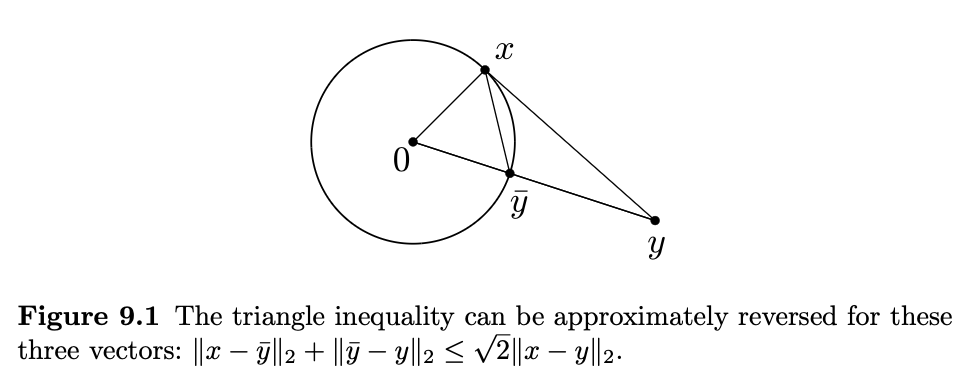
\includegraphics[width=0.8\textwidth]{Chapter 9/fig9-1.png}
\end{center}
Then by triangle inequality:
\[ \lVert Z_x - Z_y \rVert_{\psi_2} \leq \lVert Z_x - Z_{\bar{y}} \rVert_{\psi_2} 
+ \lVert Z_{\bar{y}} - Z_y \rVert_{\psi_2}. \]
Since both $x, \bar{y}$ are unit vectors, the result of Step 3 handles the first term:
\[ \lVert Z_x - Z_{\bar{y}} \rVert_{\psi_2} \leq CK^2 \lVert x - \bar{y} \rVert_{2}. \]
To handle the second term, note that $\bar{y}$ and $y$ are colinear vectors. So by homogeneity, 
\[ \lVert Z_{\bar{y}} - Z_y \rVert_{\psi_2} = \lVert \bar{y} - y \rVert_{2} \cdot \lVert Z_{\bar{y}} 
\rVert_{\psi_2}. \]
Now, since $\bar{y}$ is a unit vector, the result of Step 1 gives $\lVert Z_{\bar{y}} \rVert_{\psi_2} 
\leq CK^2$. Conbining the two terms, we conclude that 
\[ \lVert Z_x - Z_y \rVert_{\psi_2} \leq CK^2 (\lVert x - \bar{y} \rVert_{2} + \lVert \bar{y} - y \rVert_{2}). \]
At first this looks bad - we wnat to bound right hand side by $\lVert x - y \rVert_{2}$, but the triangle 
inequality goes the other way! Luckily, in our case (via the projection of $y$), the triangle inequality can be 
approximately reversed (Exercise 9.1):
\[ \lVert x - \bar{y} \rVert_{2} + \lVert \bar{y} - y \rVert_{2} \leq \sqrt{2}\lVert x - y \rVert_{2}. \]
Plugging this into the bound above, we get the desired bound:
\[ \lVert Z_x - Z_y \rVert_{\psi_2} \leq \sqrt{2}CK^2 \lVert x - y \rVert_{2}, \]
which proves the theorem.
\end{proof}

\begin{remark}[Matrix deviations from the mean]
\label{rmk:9.1.3}
A quick centering trick turns \cref{thm:9.1.1} into a deviation inequality around the mean 
$\mathbb{E}\left[ \lVert Ax \rVert_{2} \right]$ (Exercise 9.2).
\end{remark}

\begin{remark}[Matrix deviations: a high-probability bound]
\label{rmk:9.1.4}
We only stated \cref{thm:9.1.1} as an expectation bound, but we can upgrade it to a high-probability bound via 
the high-probability version of Talagrand's inequality (Exercise 8.37(b)). For any $u \geq 0$, the event 
\[ \sup_{x \in T} \left| \lVert Ax \rVert_{2} - \sqrt{m}\lVert x \rVert_{2} \right| 
\leq CK^2 [w(T) + u \cdot \mathrm{rad}(T)] \]
holds with probability at least $1 - 2 \exp{(-u^2)}$. Can you see why the above implies the expectation bound?
\end{remark}

\begin{remark}[Matrix deviations of squares]
\label{rmk:9.1.5}
If you are interested in deviations of the quadratic process $\lVert Ax \rVert_{2}^2$, we can also deduce this 
from \cref{thm:9.1.1} (Exercise 9.3):
\[ \mathbb{E}\left[ \sup_{x \in T} \left| \lVert Ax \rVert_{2}^2 - m \lVert x \rVert_{2}^2 \right| \right] 
\leq CK^4 \gamma(T)^2 + CK^2 \sqrt{m} \mathrm{rad}(T) \gamma(T). \]
\end{remark}



% ----------9.2----------
\subsection{Random Matrices, Covariance Estimation, and Johnson-Lindenstrauss}
The matrix deviation inequality has lots of useful consequences. We'll go over a few of them in this chapter!


\subsubsection{Singular Values of Random Matrices}
Applying the matrix deviation inequality for the unit Euclidean sphere $T = S^{n - 1}$ gives us the singular 
value bounds from Chapter 4.

Here is the quick check: since for the sphere we have 
\[ \mathrm{rad}(T) = 1 \text{ and } w(T) \leq \sqrt{n}, \]
the matrix deviation inequality shows that the event 
\[ \sqrt{m} - CK^2 (\sqrt{n} + u) \leq \lVert Ax \rVert_{2} \leq \sqrt{m} + CK^2 (\sqrt{n} + u) \text{ for 
all } x \in S^{n - 1} \]
holds with probability at least $1 - 2 \exp{(-u^2)}$. Then taking the min/max gives 
\[ \sqrt{m} - CK^2 (\sqrt{n} + u) \leq \sigma_n(A) \leq \sigma_1(A) \leq \sqrt{m} + CK^2 (\sqrt{n} + u) 
\text{ for all } x \in S^{n - 1}, \]
giving \cref{thm:4.6.1} in a different way.


\subsubsection{Random Projections of Sets}
From the matrix deviation inequality, we also get a sharper bound on the random projection bound in Section 7.6:

\begin{proposition}[Sizes of random projections of sets]
\label{prop:9.2.1}
Let $T \subset \mathbb{R}^n$ be a bounded set, and let $A$ be an $m \times n$ matrix with independent, isotropic 
and subgaussian rows $A_i$. Then the scaled matrix $P = \frac{1}{\sqrt{n}}A$ (a subgaussian projection) satisfies
\[ \mathbb{E}\left[ \mathrm{diam}(PT) \right] \leq \sqrt{\frac{m}{n}}\mathrm{diam}(T) + CK^2 w_s(T). \]
Here $K = \max_{i}\lVert A_i \rVert_{\psi_2}$ and $w_s(T)$ is the spherical width of $T$.
\end{proposition}


\begin{proof}
\cref{thm:9.1.1} implies via triangle inequality:
\[ \mathbb{E}\left[ \sup_{x \in T}\lVert Ax \rVert_{2} \right] \leq \sqrt{m}\sup_{x \in T}\lVert x \rVert_{2} 
+ CK^2 \gamma(T), \]
which we can rewrite in terms of the radii of $AT$ and $T$:
\[ \mathbb{E}\left[ \mathrm{rad}(AT) \right] \leq \sqrt{m}\mathrm{rad}(T) + CK^2 \gamma(T). \]
Applying this bound for the difference set $T - T$ instead of $T$ to get 
\[ \mathbb{E}\left[ \mathrm{diam}(AT) \right] \leq \sqrt{m}\mathrm{diam}(T) + 2CK^2w(T), \]
where we used \cref{lem:7.5.11} (a) to pass from Gaussian complexity to Gaussian width. Divide both sides by 
$\sqrt{n}$ completes the proof.
\end{proof}


\subsubsection{Covariance Estimation for Low-dimensional Distributions}
Let's visit the covariance estimation problem from Section 4.7. We want to estimate the population covariance 
via the sample covariance matrix $\Sigma_m = \sum_{i = 1}^{m}X_iX_i^T$.

In general, $O(n \log_{}{n})$ samples are enough (Section 5.6), but for subgaussian distributions, $m = O(n)$ 
is enough.

It gets even better for approximately low-dimensional distributions. If a distribution concentrates near a 
$r$-dimensional subspace, $m = O(r \log_{}{n})$ samples suffice (\cref{rmk:5.6.3}). Now we will show that for 
subgaussian distributions, $m = O(r)$ samples suffices:

\begin{theorem}[Covariance estimation for low-dimensional distributions]
\label{thm:9.2.2}
Let $X$ be a subgaussian random vector in $\mathbb{R}^n$. More spefically, assume that these exists $K \geq 1$ 
such that 
\[ \lVert \left\langle X, x \right\rangle \rVert_{\psi_2} \leq K \lVert \left\langle X, x 
\right\rangle \rVert_{L^2} \text{ for any } z \in \mathbb{R}^n. \]
Then, for every positive integer $m$, 
\[ \mathbb{E}\left[ \lVert \Sigma_m - \Sigma \rVert_{} \right] \leq CK^4 \left( 
\sqrt{\frac{r}{m}} + \frac{r}{m} \right) \lVert \Sigma \rVert_{}, \]
where $r = \mathrm{tr}(\Sigma)/\lVert \Sigma \rVert_{}$ is the effective rank of $\Sigma$.
\end{theorem}

\begin{proof}
We start as in \cref{thm:4.7.1} by bringing the distribution to the isotropic position: $X = \Sigma^{1/2}Z$ and 
$X_i = \Sigma^{1/2}Z_i$ where $Z$ and $Z_i$ are isotropic, and 
\begin{align*}
	\lVert \Sigma_m - \Sigma \rVert_{} 
	&= \lVert \Sigma^{1/2} E_m \Sigma^{1/2} \rVert_{} \quad (R_m = \frac{1}{m}\sum_{i = 1}^{m}Z_iZ_i^T - I_n) \\
	&= \max_{x \in S^{n-1}} |x^T \Sigma^{1/2} R_m \Sigma^{1/2} x| \quad \text{(\cref{rmk:4.1.12})} \\
	&= \max_{x \in T}|x^T R_m x| \quad (T := \Sigma^{1/2}S^{n-1}) \\
	&= \max_{x \in T} \left| \frac{1}{m}\sum_{i = 1}^{m}\left\langle Z_i, x \right\rangle^2 - 
	\lVert x \rVert_{2}^2 \right| \\
	&= \frac{1}{m}\max_{x \in T} \left| \lVert Ax \rVert_{2}^2 - m \lVert x \rVert_{2}^2 \right|,
\end{align*}
where $A$ is the $m \times n$ matrix with ros $Z_i$. As in the proof of \cref{thm:4.7.1}, $Z_i$ are isotropic, 
and satisfy $\lVert Z_i \rVert_{\psi_2} \lesssim 1$. This allows us to apply the matrix deviation inequality 
for $A$ (in the form given by Exercise 9.3), which gives
\[ \mathbb{E}\left[ \lVert \Sigma_m - \Sigma \rVert_{} \right] \lesssim 
\frac{1}{m}(\gamma(T)^2 + \sqrt{m}\mathrm{rad}(T)\gamma(T)). \]
The radius and Gaussian complexity of the ellipsoid $T = \Sigma^{1/2}S^{n-1}$ satisfy 
\[ \mathrm{rad}(T) = \lVert \Sigma \rVert_{}^{1/2} \text{ and } \gamma(T) \leq (\mathrm{tr}(\Sigma))^{1/2}. \]
Therefore, 
\[ \mathbb{E}\left[ \lVert \Sigma_m - \Sigma \rVert_{} \right] \lesssim 
\frac{1}{m} (\mathrm{tr}(\Sigma) + \sqrt{m \lVert \Sigma \rVert_{} \mathrm{tr}(\Sigma)}). \]
Substituting $\mathrm{tr}(\Sigma) = r \lVert \Sigma \rVert_{}$ and simplifying the bound completes the proof.
\end{proof}

\begin{remark}[Covariance estimation: a high-probability guarantee]
\label{rmk:9.2.4}
Just like the versions before (\cref{rmk:4.7.3} and \cref{rmk:5.6.5}), we can upgrade the expectation bound 
above to a high-probability one. For any $u \geq 0$ we have 
\[ \lVert \Sigma_m - \Sigma \rVert_{} \leq CK^4 \left( 
\sqrt{\frac{r + u}{m}} + \frac{r + u}{m} \right) \lVert \Sigma \rVert_{} \]
with probability at least $1 - 2e^{-u}$. 
\end{remark}

\begin{proof}
Exercise 9.9.
\end{proof}


\subsubsection{Johnson-Lindenstrauss Lemma for Infinite Sets}
The matrix deviation inequality quickly recovers the Johnson-Lindenstrauss lemma from Section 5.3 - and extends 
it to general, possibly infinite, sets.

To get a version of the JL lemma from matrix deviation, fix any $N$-point set $\mathcal{X} \in \mathbb{R}^n$ 
and consider the normalized differences: 
\[ T := \left\{ \frac{x - y}{\lVert x - y \rVert_{2}}: \ x, y \in \mathcal{X} \text{ distinct} \right\}. \]
The Gaussian complexity of $T$ satisfies 
\[ \gamma(T) \leq C \sqrt{\log_{}{N}}. \]
The matrix deviation inequality (\cref{thm:9.1.1}) shows that with high probability, 
\[ \sup_{x, y \in \mathcal{X}} \left| \frac{\lVert Ax - Ay \rVert_{2}}{\lVert x - y \rVert_{2}} - 
\sqrt{m} \right| \lesssim \sqrt{\log_{}{N}}. \]
Rearranging the terms, rewrite this as follows: the random matrix $Q := \frac{1}{\sqrt{m}}A$ is an approximate 
isometry on $\mathcal{X}$, i.e.
\[ (1 - \varepsilon)\lVert x - y \rVert_{2} \leq \lVert Qx - Qy \rVert_{2} \leq (1 + \varepsilon)\lVert x - y
\rVert_{2} \text{ for all } x, y \in \mathcal{X}, \]
for some $\varepsilon \asymp \sqrt{\log_{}{(N)} / m}$. Equivalently, if we fix $\varepsilon > 0$ and choose 
\[ m \gtrsim \varepsilon^{-2} \log_{}{N}, \]
then with high probability $Q$ is an $\varepsilon$-isometry on $\mathcal{X}$, which recovers a version of the 
classical JL lemma.

What we just not gave did not care if $\mathcal{X}$ is finite or not - all that matters is the Gaussian width. 
So we can extend JL to any set:

\begin{lemma}[Additive Johnson-Lindenstrauss lemma]
\label{lem:9.2.4}
Let $\mathcal{X} \subset \mathbb{R}^n$ be a bounded set, and let $A$ be an $m \times n$ matrix with independent, 
isotropic and subgaussian rows $A_i$. Then, with high probability (say 0.99), the scaled matrix $Q = 
\frac{1}{\sqrt{m}}A$ satisfies 
\[ |\lVert Qx - Qy \rVert_{2} - \lVert x - y \rVert_{2}| \leq \delta \text{ for all } x, y \in \mathcal{X} \]
where $\delta = CK^2w(\mathcal{X}) / \sqrt{m}$ and $K = \max_{i}\lVert A_i \rVert_{\psi_2}$.
\end{lemma}

\begin{proof}
Apply the matrix deviation inequality (\cref{thm:9.1.1}) for the set of differences $T = \mathcal{X}-
\mathcal{X}$. Then, with high probability, 
\[ \sup_{x, y \in \mathcal{X}} \left| \lVert Ax - Ay \rVert_{2} - \sqrt{m}\lVert x - y \rVert_{2} \right| 
\leq CK^2 \gamma(\mathcal{X}-\mathcal{X}) = 2CK^2 w(\mathcal{X}), \]
thanks to \cref{lem:7.5.11} (a). Divide both sides by $\sqrt{m}$ completes the proof.
\end{proof}

Unlike the classical JL lemma for finite sets (\cref{thm:5.3.1}), which gives a relative error, here we get an 
absolute error $\delta$. It is a small difference - but in general, a necessary one (Exercise 9.11).

\begin{remark}[Effective dimension]
\label{rmk:9.2.5}
To better understand the additive Johnson-Lindenstrauss lemma, let's restate it using the effective dimension of 
the data $d(\mathcal{X}) \asymp w(\mathcal{X})^2 / \mathrm{diam}(\mathcal{X})^2$. If we choose 
\[ m \gtrsim \varepsilon^{-2} d(T) \]
(ignoring the dependence on $K$ for simplicity), then we can make $\delta = \varepsilon \mathrm{diam}
(\mathcal{X})$, so $Q$ preserves distances up to a small fraction of diameter - in other words, it reduces the 
dimension of the data down to its effective dimension.
\end{remark}



% ----------9.3----------
\subsection{Random Sections: The \texorpdfstring{$M^*$}{} Bound and Escape Theorem}
Here is a surprising high-dimensional fact: if you slice a convex set $T \subset \mathbb{R}^n$ with a random 
subspace $E$ of codimension $m$, the slice $T \subset E$ is often tiny - even when $m \ll n$ and $E$ is near 
full-dimensional! Let's see how this follows from the matrix deviation inequality.


\subsubsection{The \texorpdfstring{$M^*$}{} Bound}
It is handy to model a random subspace $E$ as the kernel of an $m \times n$ random matrix: $E = \ker{A}$. We 
always have 
\[ \dim{(E)} \geq n - m, \]
and if $A$ has a continuous distribution, $\dim{(E)} \geq n - m$ almost surely.

A great example is a Gaussian matrix $A$ with i.i.d. $N(0, 1)$ entries - by rotation invariance, $E - \ker{(A)}$ 
is uniformly distributed in the Grassmannian:
\[ E \sim \mathrm{Unif}(G_{n, n - m}). \]

\begin{theorem}[$M^*$ bound]
\label{thm:9.3.1}
Let $T \subset \mathbb{R}^n$ be a bounded set, and $A$ be an $m \times n$ random matrix with independent, 
isotropic and subgaussian rows $A_i$. Then the random subspace $E = \ker{A}$ satisfies 
\[ \mathbb{E}\left[ \mathrm{diam}(T \cap E) \right] \leq \frac{CK^2 w(T)}{\sqrt{m}}, \]
where $K = \max_{i}\lVert A_i \rVert_{\psi_2}$.
\end{theorem}

\begin{proof}
Apply \cref{thm:9.1.1} for $T - T$:
\[ \mathbb{E}\left[ \sup_{x, y \in T} \left| \lVert Ax - Ay \rVert_{2} - \sqrt{m}\lVert x - y \rVert_{2} \right| 
\leq CK^2 \gamma(T - T) = 2CK^2 w(T), \right] \]
by \cref{lem:7.5.11} (a). Considering only the points $x, y$ in the kernel of $A$ makes $\lVert Ax - Ay 
\rVert_{2}$ disappear since $Ax = Ay = 0$. Divide both sides by $\sqrt{m}$ to get 
\[ \mathbb{E}\left[ \sup_{x, y \in T \cap \ker{A}} \lVert x - y \rVert_{2} \right] 
\leq \frac{CK^2 w(T)}{\sqrt{m}}, \]
which is exactly what we claimed.
\end{proof}

\begin{example}[The cross-polytope]
Let's apply the $M^*$ bound to the cross-polytope $B_1^n$ - the unit ball of the $\ell^1$ norm. Since its 
Gaussian width id roughly $\sqrt{\log_{}{n}}$ by \cref{ex:7.5.8}, we get 
\[ \mathbb{E}\left[ \mathrm{diam}(B_1^n \cap E) \right] \lesssim \sqrt{\frac{\log_{}{n}}{m}}. \]
For example, if $m = 0.01n$, then 
\[ \mathbb{E}\left[ \mathrm{diam}(T \cap E) \right] \lesssim \sqrt{\frac{\log_{}{n}}{n}}. \]
So, a random $0.99n$-dimensional slice of a cross-polytope is tiny!
\end{example}

How can this be? This relates to what we discussed in \cref{rmk:7.5.10}. The ``bulk" of $B_1^n$ is concentrated 
near the inscribed ball of radius $1/\sqrt{n}$, while the rest stretches out into long, thin ``spikes" along 
the coordinate axes. A random subspace $E$ probably misses those spikes and cuts through the bulk (Figure 9.2a). 
Therefore the slice ends up with diameter about $O(1/\sqrt{n})$, maybe with a log factor as shown above. This 
intuition can be extended to general convex sets as well.

\begin{center}
	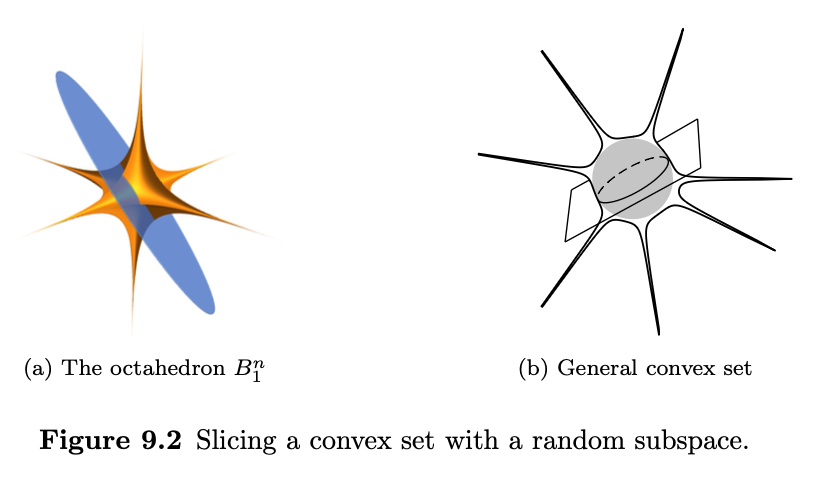
\includegraphics[width=0.8\textwidth]{Chapter 9/fig9-2.png}
\end{center}

\begin{remark}[Effective dimension]
\label{rmk:9.3.3}
To get more intuition, write the $M^*$ bound using the effective dimension (\cref{def:7.5.12}). The $M^*$ bound 
shows that slicing shrinks the dimaeter:
\[ \mathbb{E}\left[ \mathrm{diam}(T \cap E) \right] \leq 0.01 \cdot \mathrm{diam}(T) \]
as long as $m \gtrsim d(T)$. Since $\dim{(E)} = n - m$, this condition is equivalent to 
\[ \dim{(E)} + cd(T) \leq n. \]
That lines up with the linear algebra intuition: If $T$ is a cnetered Euclidean ball in some subspace 
$F \subset \mathbb{R}^n$, slicing can shrink the diameter of $T$ only when $\dim{E} + \dim{F} \leq n$.
\end{remark}


\subsubsection{The Escape Theorem}
When does a random subspace $E$ miss a given set $T$ entirely with high probability? Not if $T$ contains the 
origin - but if $T$ lies on the unit sphere (Figure 9.3), then it does as long as the codimension of $E$ is not 
too small: 

\begin{center}
	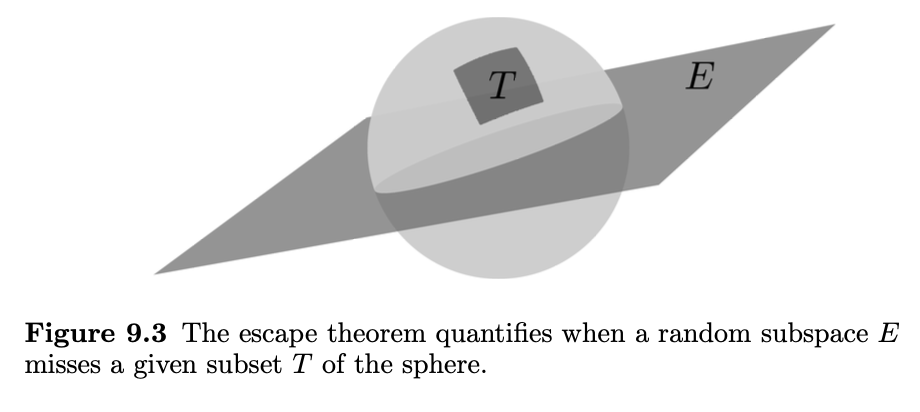
\includegraphics[width=0.8\textwidth]{Chapter 9/fig9-3.png}
\end{center}

\begin{theorem}[Escape theorem]
\label{thm:9.3.4}
Let $T \subset S^{n - 1}$ be any set, and let $A$ be an $m \times n$ matrix with independent, isotropic and 
subgaussian rows $A_i$. If 
\[ m \geq CK^4 w(T)^2, \]
then the random subspace $E = \ker{A}$ satisfies 
\[ T \cap E = \emptyset \]
with probability ar least $1 - 2 \exp{(-cm/K^4)}$. Here $K = \max_{i}\lVert A_i \rVert_{\psi_2}$.
\end{theorem}

\begin{proof}
Let us use the high-probability version of the matrix deviation inequality (\cref{rmk:9.1.4}): With probability 
at least $1 - 2 \exp{(-u^2)}$, 
\[ \sup_{x \in T}\left| \lVert Ax \rVert_{2} - \sqrt{m} \right| \leq C_1K^2(w(T) + u). \]
Suppose the above occurs. If $T \cap E \neq \emptyset$, then for any $x \in T \cap E$ we have $Ax = 0$, so 
\[ \sqrt{m} \leq C_1 K^2 (w(T) + u). \]
Set $u = \sqrt{m}/(2C_1K^2)$ and simplify this bound to get 
\[ \sqrt{m} \leq 2 C_1 K^2 w(T), \]
which contradicts the assumption if $C$ is large enough.Therefore, with that choice of $u$, the event implies 
$T \cap E = \emptyset$. Done!
\end{proof}


% ----------9.4----------
\subsection{Application: High-dimensional Linear Models}
Let's apply our tools on a classic data science problem: learning a linear model in high dimensions. Let 
\[ y_i = \left\langle A_i, x \right\rangle + w_i, \ i = 1, \dots, m. \]
Her $A_i \in \mathbb{R}^n$ are known, and $w_i$ are unknown numbers representing noise (Figure 9.4). In matrix form, we get 
\[ y = Ax + w. \]
The goal is to recover $x$ from $y$ and $A$ as accurately as possible. 

\begin{center}
	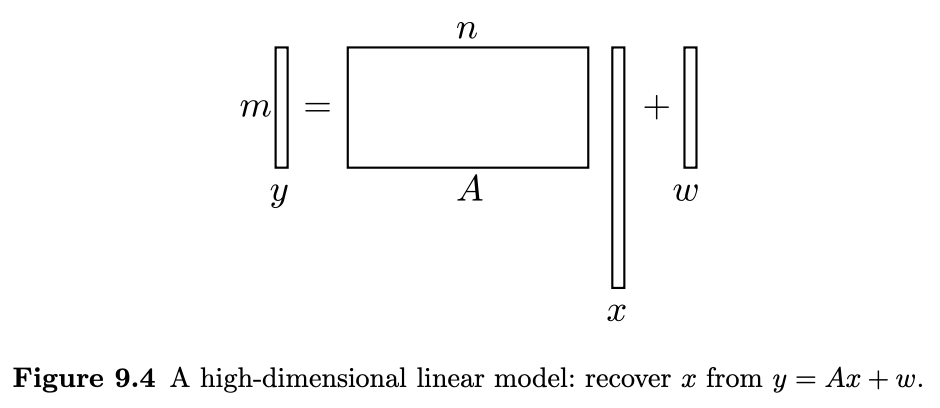
\includegraphics[width=0.8\textwidth]{Chapter 9/fig9-4.png}
\end{center}

We assume the rows $A_i$ of $A$ are random and independent - this is reasonable in many statistical settings 
(think about i.i.d. observations), and perfect for applying tools from high-dimensional probability.

\begin{example}[Audio sampling]
\label{ex:9.4.1}
In signal processing, $x$ could be a digitized audio signal, and $y$ the result of sampling it at $m$ random 
time points (Figure 9.5).

\begin{center}
    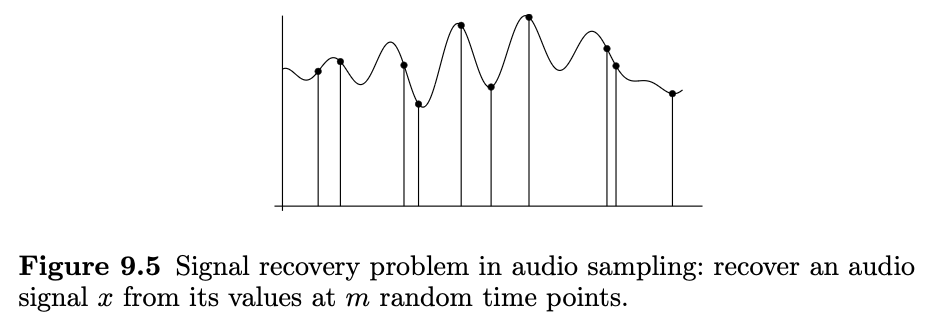
\includegraphics[width=0.8\textwidth]{Chapter 9/fig9-5.png}
\end{center}
\end{example}

\begin{example}[Linear regression]
\label{ex:9.4.2}
A core porblem in statistics is linear regression, where we want to learn a linear relationship between $n$ 
predictor variables and a response variable from $m$ samples. It is written as 
\[ Y = X \theta + w \]
where $X$ is an $m \times n$ matrix of predictors, $Y \in \mathbb{R}^m$ is the vector of responses, $\theta \in 
\mathbb{R}^n$ is the parameter vector that we are trying to learn.
\end{example}

\begin{remark}[The high-dimensional regime]
\label{rmk:9.4.3}
In modern problems, we often have less data than parameters: 
\[ m \ll n, \]
For example, in a genetic study, there might be $\sim$100 patients, but $\sim$10000 genes. In this 
high-dimensional setting, even solving $Ax  = y$ becomes impossible, as there are too many possible solutions 
as they live in a large subspace of dimension at least $m - n$.

Not all hope is lost. If we have some prior information about the structure of $x$, which we can write this as 
\[ x \in T \]
for some known set $T \subset \mathbb{R}^n$, then we might be able to recover $x$. For example, if $x$ is 
sparse, we can pick $T$ to be the set of all sparse vectors.
\end{remark}


\subsubsection{Constrained Recovery}
Let's solve the noiseless case first:
\[ y = Ax, \ x \in T. \]
How do we solve this dimensional constrained linear problem?

A simple idea is just to pick any vector $x' \in T$ that matches the observations:
\[ \text{find } x': \ y = Ax', \ x \in T. \]
If $T$ is convex, this is a convex program, and many algorithms exist to numerically solve it. Let's check 
how accurate this solution is.

\begin{theorem}[Constrained recovery]
\label{thm:9.4.4}
Suppose the rows $A_i$ of $A$ are independent, isotropic and subgaussian random vectors. Then any solution 
$\Hat{x}$ of the convex linear program satisfies 
\[ \mathbb{E}\left[ \lVert \Hat{x} - x \rVert_{2} \right] \leq \frac{CK^2 w(T)}{\sqrt{m}}, \]
where $K = \max_{i}\lVert A_i \rVert_{\psi_2}$.
\end{theorem}

\begin{proof}
Since $x, \Hat{x} \in T$ and $Ax = A \Hat{x} = y$, we have 
\[ x, \Hat{x} \in T \cap E_x, \text{ where } E_x = x + \ker{A} \]
See Figure 9.6 for an illustration.

\begin{center}
    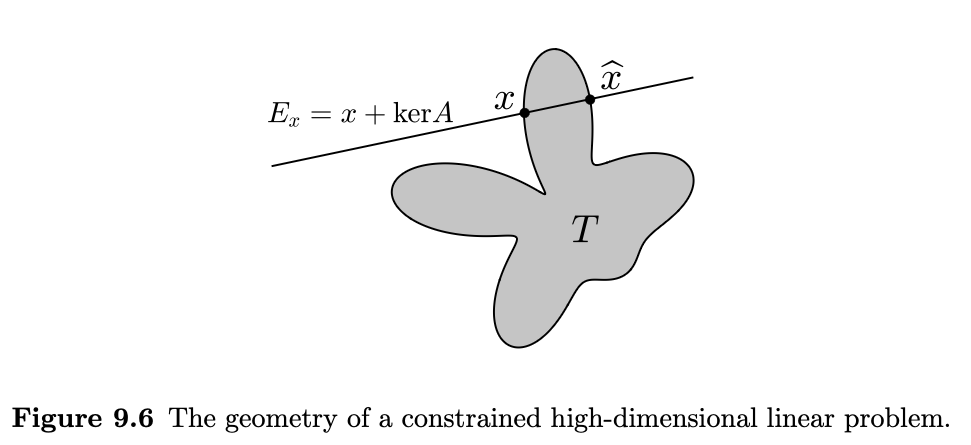
\includegraphics[width=0.8\textwidth]{Chapter 9/fig9-6.png}
\end{center}
Then the $M^*$ bound (in the form of Exercise 9.12) gives 
\[ \mathbb{E}\left[ \lVert \Hat{x} - x \rVert_{2} \right] 
\leq \mathbb{E}\left[ \mathrm{diam}(T \cap E_x) \right] \leq \frac{CK^2 w(T)}{\sqrt{m}}. \]
\end{proof}

\begin{remark}[Effective dimension]
\label{rmk:9.4.5}
To get some intuition, rewrite the accuracy guarantee in \cref{thm:9.4.4} using the effective dimension 
(\cref{def:7.5.12}). We get a nontrivial error bound 
\[ \mathbb{E}\left[ \lVert \Hat{x} - x \rVert_{2} \right] \leq 0.01 \mathrm{diam}(T) \]
as long as the number of observations satisfies (suppressing $K$ again)
\[ m \gtrsim d(T). \]
Since $d(T)$ can be much smaller than the ambient dimension $n$, recovery is often possible even in the 
high-dimensional regime.
\end{remark}

\begin{remark}[Convex relaxation]
\label{rmk:9.4.6}
If $T$ is not convex, we can just use its convex hull $\mathrm{conv}(T)$. The recovery guarantees from 
\cref{thm:9.4.4} do not change, as $w(\mathrm{conv}(T)) = w(T)$ by \cref{prop:7.5.2} (c).
\end{remark}

\begin{remark}[Unconstrained optimization]
\label{rmk:9.4.7}
Forcing strict rules on the solution like $y = Ax'$ and $x' \in T$ can be too rigid - noise or a bad choice for 
$T$ might mean no solution exists. Instead, we could aim to penalize how much they are broken by solving the 
unconstrained convex problem 
\[ \min_{}\lVert y - Ax \rVert_{2}^2 + \lambda \lVert x \rVert_{T}, \ x \in \mathbb{R}^n, \]
where $\lVert \cdot \rVert_{T}$ is any norm you like, and $\lambda > 0$ is a parameter we can adjust to see 
which summand we want to prioritize more.
\end{remark}


We also have the following guarantee from Exercise 9.20: if $A$ is an $m \times n$ random matrix, and $\lambda$ 
is chosen well, then the solution $\Hat{x}$ satisfies 
\[ \mathbb{E}\left[ \lVert \Hat{x} - x \rVert_{2} \right] \lesssim 
\frac{w(T)\lVert x \rVert_{T} + \lVert w \rVert_{2}}{\sqrt{m}}, \]
where $T$ is the unit ball of $\lVert \cdot \rVert_{T}$. 

In short, if $x$ is well structured and the noise $w$ is small, then you can recover $x$ accurately from 
$m \asymp d(T)$ observations, where $d(T)$ is the effective dimension of $T$.


\subsubsection{Example: Sparse Recovery}
Sometimes we believe that $x$ is \textit{sparse} - most of its entries are zero or nearly zero. We can 
quantify the sparsity of $x \in \mathbb{R}^n$ by the number of nonzero entries:
\[ \lVert x \rVert_{0} = |\mathrm{supp}(x)| = |\{ i: \ x_i \neq 0 \}|, \]
and we say that $x$ is sparse if $\lVert x \rVert_{0} \leq s$. The ``$\ell^0$ norm" is not really a norm, but 
is a limit of $\ell^p$ norms as $p \to 0$ (Exercise 9.23).

A quick dimension count shows that we can recover $x$ from $y = Ax$ if $A$ is in a general position and we have 
enough observations: $m \geq 2 \lVert x \rVert_{0}$ (Exercise 9.22). Sounds great, as we can recover a sparse 
vector from only a few observations. The catch? It's computationally hard unless we already know the support of 
$x$. Without that, the best way is to brute force - $\binom{n}{s} \geq 2^s$ subsets to check!

To solve this, we can pick the prior using the $\ell^1$ norm, the closest $\ell^p$ that is actually a norm 
(Exercise 9.23). Since $s$-sparse vectors with $\lVert x \rVert_{2} \leq 1$ satisfy $\lVert x \rVert_{2} \leq 
\sqrt{s}$, it makes sense to pick the convex set 
\[ T := \sqrt{s}B_1^n \]
as our prior. The recovery program becomes 
\[ \text{find } x: \ y = Ax, \ \lVert x \rVert_{1} \leq \sqrt{s}. \]

\begin{corollary}[Sparse recovery]
\label{cor:9.4.8}
Suppose the rows $A_i$ of $A$ are independent, isotropic and subgaussian random vectors. Assume an unknown 
$s$-sparse vector $x \in \mathbb{R}^n$ satisfies $\lVert x \rVert_{2} \leq 1$. Then any solution $\Hat{x}$ to 
the program above satisfies 
\[ \mathbb{E}\left[ \lVert \Hat{x} - x \rVert_{2} \right] \leq CK^2 \sqrt{\frac{s \log_{}{n}}{m}}, \]
where $K = \max_{i}\lVert A_i \rVert_{\psi_2}$.
\end{corollary}

\begin{proof}
Set $T = \sqrt{s}B_1^n$. Then the result follows from \cref{thm:9.4.4} and the bound on the Gaussian width 
of the $\ell^1$ ball: 
\[ w(T) = \sqrt{s}w(B_1^n) \leq C \sqrt{s \log_{}{n}}. \]
\end{proof}

\begin{remark}[Observations scale almost linearly with sparsity]
\label{rmk:9.4.9}
\cref{cor:9.4.8} gives a small error as long as
\[ m \gtrsim s \log_{}{n} \]
(if the hidden constant is appropriately large). That's great news - we can efficiently recover a sparse vector 
from way fewer observations $m$ than the full dimension $n$.
\end{remark}

\begin{remark}[A logarithmic improvement]
\label{rmk:9.4.10}
The set $S_{n, s}$ of unit $s$-sparse vectors in $\mathbb{R}^n$ can be convexified a bit tighter. Instead of 
using the $\ell^1$ ball, use the \textit{truncated} $\ell^1$ ball 
\[ T_{n,s} = \sqrt{s}B_1^n \cap B_2^n. \]
This relaxation is pretty tight - Exercise 9.25 gives 
\[ \mathrm{conv}(S_{n,s}) \subset T_{n,s} \subset 2\mathrm{conv}(S_{n,s}).  \]
This tightening gives a logarithmic improvement on the bound in \cref{cor:9.4.8}, showing that 
\[ m \gtrsim s \log_{}{(en/s)} \]
observations suffice for sparse recovery (Exercise 9.21).
\end{remark}


\subsubsection{Example: Low-rank Recovery}
Here is one more example of a high-dimensional linear problem: recover a $d \times d$ matrix $X$ (instead of 
a vector) from $m$ linear observations:
\[ y_i = \left\langle A_i, X \right\rangle, \ i = 1, \dots, m, \]
where $A_i$ are known, independent random matrices, adn the inner product is 
\[ \left\langle A, B \right\rangle = \mathrm{tr}(A^T B). \]

Normally, we would need $d^2$ observations - one per entry. To get away with fewer, we need some structure in 
$X$. A common one is low rank. Just like sparsity counts nonzero entries, rank counts nonzero singular values.

In section 9.4.2, we took a relaxation by replacing the $\ell^0$ norm with the $\ell^1$ norm. Here we'll use 
a convex relaxation by replacing the $\ell^0$ norm for the singular values with the $\ell^1$ norm, which 
is also known as the \textit{nuclear norm}:
\[ \lVert X \rVert_{*} := \sum_{i = 1}^{d} \sigma_i(X). \]

Since every vector $x$ with at most $s$ nonzero entries and $\lVert x \rVert_{2} \leq 1$ satisfies 
$\lVert x \rVert_{} \leq \sqrt{s}$, every matrix with rank at most $r$ and $\lVert X \rVert_{F} = 1$ satisfies 
\[ \lVert X \rVert_{*} \leq \sqrt{r}. \]
Therefore, it makes sense to consider $T = \sqrt{r}B_*$ as our prior, where 
\[ B_* = \{ X \in \mathbb{R}^{d \times d}: \ \lVert X \rVert_{*} \leq 1 \}. \]
Then, the recovery program becomes 
\[ \text{find } X: \ y_i = \left\langle A_i, X \right\rangle \forall i; \ \lVert X \rVert_{*} \leq \sqrt{r}, \]
which is convex and computationally tractable. And \cref{thm:9.4.4} gives 

\begin{corollary}[Low-rank matrix recovery]
\label{cor:9.4.11}
Suppose $A_i$ are independent Gaussian random matrices with all i.i.d. $N(0, 1)$ entries. Assume an unknown 
$d \times d$ matrix $X$ has rank at most $r$ and $\lVert X \rVert_{F} \leq 1$. Then any solution $\Hat{X}$ of 
the program satisfies 
\[ \mathbb{E}\left[ \lVert \Hat{X} - X \rVert_{F} \right] \leq C \sqrt{\frac{rd}{m}}. \]
\end{corollary}

\begin{proof}
Using the duality between the nuclear and operator norms (Exercise 7.18a), we get that for a $d \times d$ 
Gaussian matrix $G$ with i.i.d. $N(0, 1)$ entries:
\[ w(B_*) = \mathbb{E}\left[ \sup_{\lVert X \rVert_{*} \leq 1} \left\langle G, X \right\rangle \right] 
= \mathbb{E}\left[ \lVert G \rVert_{} \right] \leq 2 \sqrt{d} \]
by \cref{thm:7.3.1}. Now just apply \cref{thm:9.4.4} with $T = \sqrt{r}B_*$. 
\end{proof}

\begin{remark}[Recovering a low-rank matrix from few observations]
\label{rmk:9.4.12}
\cref{cor:9.4.8} gives a small error as long as
\[ m \gtrsim rd, \]
allowing us to recover a low-rank matrix from war fewer observations $m$ then the entirety $d^2$. This is 
similar to the matrix completion problem in Section 6.5, where we can recover a low-rank matrix from about 
$m \asymp rd \log_{}{d}$ randomly chosen entries.
\end{remark}



% ----------9.5----------
\subsection{Application: Exact Sparse Recovery}
In the noiseless case, we can do even better - we can recover a sparse vector $x$ from $y = Ax$ \textit{exactly} 
(and algorithmically effective)! We will look at two ways to get this surprising result:
\begin{enumerate}
	\item Use the escape theorem (\cref{thm:9.3.4}).
	\item Using the restricted isometry property - then show random matrices satisfy it with high probability.
\end{enumerate}


\subsubsection{Exact Recovery Based on the Escape Theorem}
Let's look at Figure 9.7 below for some intuition.

\begin{center}
	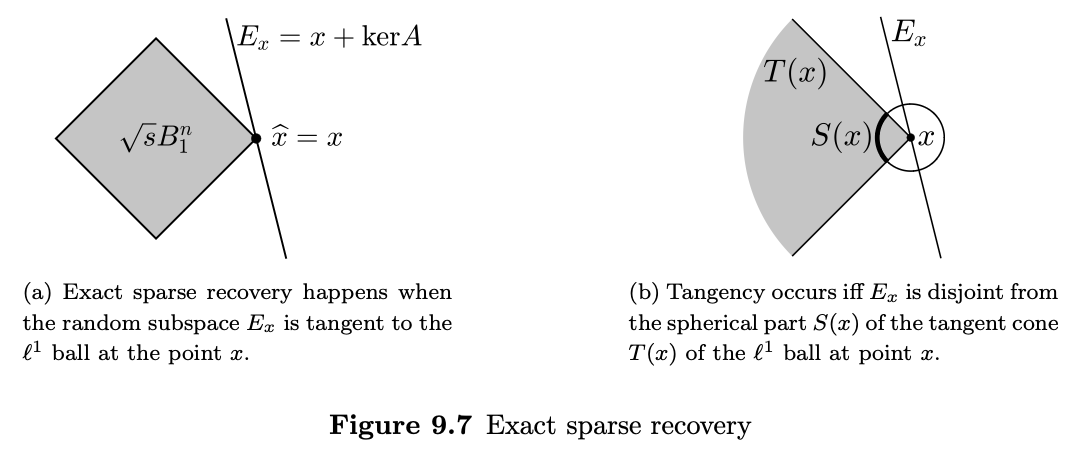
\includegraphics[width=0.8\textwidth]{Chapter 9/fig9-7.png}
\end{center}

Suppose we are trying to recover an unknown $s$-sparse unit vector $x$ from $y=Ax$ by solving the convex program 
in Section 9.4.2. A solution $\Hat{x}$ lies in the intersection of the prior set $T = \sqrt{s}B_1^n$ and the 
affine subspace $E_x = x + \ker{A}$.

$T$ is a cross-polytope, and $x$ sits on one of its $(s-1)$-dimensional edges (Figure 9.7a). With some 
probability, the random subspace $E_x$ is tangent to the polytope at $x$. If so, $x$ is the only point where 
$T$ and $E_x$ intersect, hence the solution $\Hat{x}$ must be exact:
\[ \Hat{x} = x. \]
To justify this argument, we just need to show that a random subspace $E_x$ is tangent to the $\ell^1$ ball 
with high probability. That's where the escape theorem (\cref{thm:9.3.4}) comes in. Zoom in near $x$
(Figure 9.7b): $E_x$ is tangent if and only if the \textit{tangent cone} $T(x)$ (all rays coming from x into 
the $\ell^1$ ball) intersects $E_x$ only at $x$. This happens if the \textit{spherical part} $S(x)$ of the 
cone (the intersection of $T(x)$ with a small sphere centered at $x$) is disjoint from $E_x$ – and that is 
exactly what the escape theorem can guarantee!

Let's formalize this. We want to recover $x$ from 
\[ y = Ax \]
by solving the optimization problem 
\[ \min_{}\lVert x \rVert_{1} \text{ subject to } y = Ax. \]

\begin{theorem}[Exact sparse recovery]
\label{thm:9.5.1} A $m \times n$ matrix $A$ with independent, isotropic, subgaussian rows $A_i$ satisfies the 
following with probability at least $1 - 2 \exp{(-cm/K^4)}$, where $K = \max_{i}\lVert A_i \rVert_{\psi_2}$:

If the number of observations satisfies 
\[ m \geq CK^4 s \log_{}{n}, \]
then for any $s$-sparse vector $x \in \mathbb{R}^n$, a solution $\Hat{x}$ of the convex program is exact:
\[ \Hat{x} = x. \]
\end{theorem}

To prove this, we want to show that the recovery error is 0:
\[ h := \Hat{x} - x = 0. \]
First, let's show a weaker claim: $h$ has more mass on the spport of $X$ than off it.

\begin{lemma}[The error is heavier on $x$'s support]
\label{lem:9.5.2}
Set $S := \mathrm{supp}(x)$, and let $h_S \in \mathbb{R}^S$ denote the restriction of $h$ onto $S$ (and 
similartly for $S^c$). Then 
\[ h_{S^c} \leq \lVert h_S \rVert_{1}. \]
\end{lemma}

\begin{proof}
Since $\Hat{x}$ is the minimizer in the program, we have 
\[ \lVert \Hat{x} \rVert_{1} \leq \lVert x \rVert_{1}. \]
But there is also a lower bound
\begin{align*}
	\lVert \Hat{x} \rVert_{1} 
	&= \lVert x + h \rVert_{1} \\
	&= \lVert x_S + h_S \rVert_{1} + \lVert x_{S^c} + h_{S^c} \rVert_{1} \\
	&\geq \lVert x \rVert_{1} - \lVert h_S \rVert_{1} + \lVert h_{S^c} \rVert_{1},
\end{align*}
where the last line follows by triangle inequality and using $x_S = x$ and $x_{S^c} = 0$. Substituting this 
into the first equation completes the proof.
\end{proof}

\begin{lemma}[The error is approximately sparse]
\label{lem:9.5.3}
The error vector satisfies 
\[ \lVert h \rVert_{1} \leq 2 \sqrt{s}\lVert h \rVert_{2}. \]
\end{lemma}

\begin{proof}
Using \cref{lem:9.5.2} and then the Cauchy-Schwartz inequality, we get 
\begin{align*}
	\lVert h \rVert_{1} 
	&= \lVert h_S \rVert_{1} + \lVert h_{S^\subset1} \rVert_{1} \\
	&\leq 2 \lVert h_S \rVert_{1} \\
	&\leq 2 \sqrt{s}\lVert h_S \rVert_{2} \\
	&\leq 2 \sqrt{s}\lVert h \rVert_{2}.
\end{align*}
\end{proof}

Now let's return to the proof for exact sparse recovery.
\begin{proof}[Proof of \cref{thm:9.5.1}]
Assume $h = \Hat{x} - x \neq 0$. \cref{lem:9.5.3} gives 
\[ \frac{h}{\lVert h \rVert_{2}} \in T_s := \{ z \in S^{n-1}: \ \lVert z \rVert_{1} \leq 2 \sqrt{s} \}. \]
Since also $Ah = A \Hat{x} - Ax = y - y = 0$, we have 
\[ \frac{h}{\lVert h \rVert_{2}} \in T_s \cap \ker{A}. \]
The escape theorem (\cref{thm:9.3.4}) shows that this intersection is empty with high probability as long as 
$m \geq C_1 K^4w(T_s)^2$. Now, since $T_s \subset 2 \sqrt{s}B_1^n$, we get
\[ w(T_s) \leq 2 \sqrt{s} w(B_1^n) \leq C_2 \sqrt{s \log_{}{n}}. \]
Thus, if $m \geq CK^4s \log_{}{n}$, the intersection $T_s \cap \ker{A}$ is empty with high probability, which 
means the inclusion in the first equation cannot hold. Therefore, our assumption that $h \neq 0$ is false 
with high probablity, and the proof is complete.
\end{proof}

\begin{remark}[Improving the logarithmic factor]
\label{rmk:9.5.4}
By slightly tightening the last equation from \cref{lem:9.5.3}, we can improve the number of sufficient 
observations in \cref{thm:9.5.1} to
\[ m \geq CK^4 s \log_{}{(en/s)}. \]
This follows from Exercise 9.26.
\end{remark}


\subsubsection{Restricted Isometries}
We'll now find a \textit{deterministic} condition that ensures a matrix $A$ works for sparse recovery, and 
prove that random matrices satisfy this condition. 

\begin{definition}[]
\label{def:9.5.5} 
An $m \times n$ matrix $A$ satisfies the \underline{restricted isometry property/RIP} with 
parameters $\alpha, \beta$, and $s$ if the inequality
\[ \alpha \leq \lVert v \rVert_{2} \leq \lVert Av \rVert_{2} \leq \beta \lVert v \rVert_{2} \]
holds for all vectors $v \in \mathbb{R}^n$ with at most $s$ nonzero entries.
\end{definition}

RIP just says that the singular values of all $m \times s$ submatrices $A_I$ of $A$ satisfy 
\[ \alpha \leq \sigma_s(A_I) \leq \sigma_1(A_i) \leq \beta. \]
And if $\alpha \approx \beta \approx 1$, then RIP tells us that all those submatrices are approximate 
isometries.

\begin{theorem}[RIP implies exact recovery]
\label{thm:9.5.6}
Suppose a $m \times n$ matrix $A$ satisfies TIP with some parameters $\alpha, \beta$, and $(1 + \lambda)s$, 
where $\lambda > (\beta/\alpha)^2$. Then every $s$-sparse vector $x \in \mathbb{R}^n$ can be exactly recovered 
from $y = Ax$ by solving the convex relaxation problem earlier.
\end{theorem}

\begin{proof}
As in the proof of \cref{thm:9.5.1}, we need to show that the error
\[ h = \Hat{x} - x \]
is zero. To do this, we decompose $h$ in a way ver similar to Exercise 9.25.

\textbf{Step 1: Decomposing the support.} Let $I_0$ be the support of $x$. Let $I_1$ index the $\lambda s$ 
largest entries of $h_{I_0^c}$ in magnitude, let $I_2$ index the next $\lambda s$ largest entries of 
$h_{I_0^c}$ in magnitude, and so on. Finally, set $I_{01} = I_0 \cup I_1$. Since 
\[ Ah = A \Hat{x} - Ax = y - y = 0, \]
the triangle inequality gives 
\[ 0 = \lVert Ah \rVert_{2} \geq \lVert A_{I_{01}}h_{I_{01}} \rVert_{2} - 
\lVert A_{I_{01}^c}h_{I_{01}^c} \rVert_{2}. \quad (*) \]
Next, let's look at the two terms on the right hand side.

\textbf{Step 2: Applying RIP.} Since $|I_{0,1}| \leq s + \lambda s$, RIP gives 
\[ \lVert A_{I_{01}} h_{I_{01}} \rVert_{2} \geq \alpha \lVert h_{I_{01}} \rVert_{2} \]
and the triangle inequality followed by RIP gives 
\[ \lVert A_{I_{01}^c}h_{I_{01}^c} \rVert_{2} \leq \sum_{i \geq 2}^{} \lVert A_{I_i}h_{I_i} \rVert_{2} 
\leq \beta \sum_{i \geq 2}^{} \lVert h_{I_i} \rVert_{2}. \]
Plugging into $(*)$ gives 
\[ \beta \sum_{i \geq 2}^{}\lVert h_{I_i} \rVert_{2} \geq \alpha \lVert h_{I_{0,1}} \rVert_{2}. \quad (**) \]

\textbf{Step 3: Summing up.} Nextm we bound the sum in the left like we did in Exercise 9.25. By definition 
of $I_i$, each entry of $h_{I_i}$ is bounded in magnitude by the average of the entries of $h_{I_{i - 1}}$, 
i.e. by $\frac{1}{\lambda_s}\lVert h_{I_{i-1}} \rVert_{1}$ for $i \geq 2$. Thus 
\[ \lVert h_{I_i} \rVert_{2} \leq \frac{1}{\sqrt{\lambda s}} \lVert h_{I_{i-1}} \rVert_{1}. \]
Summing up, we get 
\begin{align*}
	\sum_{i \geq 2}^{}\lVert h_{I_i} \rVert_{2} 
	&\leq \frac{1}{\sqrt{\lambda s}}\sum_{i \geq 1}^{}\lVert h_{I_i} \rVert_{1} \\
	&= \frac{1}{\sqrt{\lambda s}} \lVert h_{I_0^c} \rVert_{1} \\
	&\leq \frac{1}{\sqrt{\lambda s}} \lVert h_{I_0} \rVert_{1} \quad \text{(\cref{lem:9.5.2})} \\
	&\leq \frac{1}{\sqrt{\lambda}} \lVert h_{I_0} \rVert_{2} \\
	&\leq \frac{1}{\sqrt{\lambda}} \lVert h_{I_{0,1}} \rVert_{2}.
\end{align*}
Putting this into $(**)$, we get 
\[ \frac{\beta}{\sqrt{\lambda}}\lVert h_{I_{0,1}} \rVert_{2} \geq \alpha \lVert h_{I_{0,1}} \rVert_{2}. \]
But this implies that $h_{I_{0,1}} = 0$ since $\beta/\sqrt{\lambda} < \alpha$ by assumption. And since 
$I_{0,1}$ contains the largest entries of $h$, it must be that $h = 0$.
\end{proof}

While we do not know how to construct deterministic matries $A$ that satisfy RIP with good parameters, we can 
show that random matrices satisfy it with high probability:

\begin{theorem}[Random matrices satisfy RIP]
\label{thm:9.5.7}
Consider an $m \times n$ matrix $A$ with independent, isotropic, subgaussian rows $A_i$. Assume that 
\[ m \geq CK^4 s \log_{}{(en/s)} \]
where $K = \max_{i} \lVert A_i \rVert_{\psi_2}$. Then, with probability at least $1 - 2 \exp{(-cm/K^4)}$, 
the random matrix $A$ satisfies RIP with paremeters 
\[ \alpha = 0.9 \sqrt{m}, \beta = 1.1 \sqrt{m}, \text{ and } s. \]
\end{theorem}

\begin{proof}
We need to check that 
\[ \alpha \leq \sigma_s(A_I) \leq \sigma_1(A_i) \leq \beta. \]
for all $m \times s$ submatrices $A_I$. First, fix $I$. By \cref{thm:4.6.1}, we get 
\[ 0.9 \sqrt{m} \leq \sigma_s(A_I) \leq \sigma_1(A_I) \leq 1.1 \sqrt{m} \]
with probability at least $1 - 2 \exp{(-cm/K^4)}$ (set $t = \sqrt{2cm}/K$ and use the assumption on $m$, 
with constants $c$ and $C$ chosen appropriately).

Now take a union bound over all $\binom{n}{s}$ possible $s$-element subsets $I \subset \{ 1, \dots, n \}$. 
Then the above holds with probability at least 
\[ 1 - 2 \exp{(-cm/K^4)} \cdot \binom{n}{s} > 1 - 2 \exp{(-cm/K^4)}, \]
using the bound $\binom{n}{s} \leq \exp{(s \log_{}{(en/s)})}$ from Exercise 0.6 and the assumption on $m$. 
Hence the proof is complete.
\end{proof}

In fact, we just learned an alternative approach to exact recovery:

\begin{proof}[Second proof of \cref{thm:9.5.1}]
By \cref{thm:9.5.7}, $A$ satisfies RIP with $\alpha = 0.9 \sqrt{m}$, $\beta = 1.1 \sqrt{m}$, and $3s$. Thus, 
\cref{thm:9.5.6} for $\lambda = 2$ guarantees exact recovery. The proof is complete. We even get the 
logarithmic improvement from Exercise 9.5.4!
\end{proof}



% ----------9.6----------
\subsection{Deviations of Random Matrices for General Norms}
We can generalize the matrix deviation inequality (\cref{thm:9.1.1}) to work for any norm - not just the 
Euclidean one. Actually we don't even need the norm to be nonnegative - just homogeneity and triangle inequality 
is enough.

\begin{definition}[]
\label{def:9.6.1}
A real-valued function $f$ on a linear vector space $V$ is called:
\begin{itemize}
	\item \underline{Positive-homogeneous} if $f(\alpha x) = \alpha f(x)$ for all $\alpha \geq 0$ and $x \in V$;
	\item \underline{Subadditive} if $f(x + y) \leq f(x) + f(y)$ for all $x, y \in V$.
\end{itemize}
\end{definition}

\begin{example}[]
\label{ex:9.6.2}
These functions are positive-homogeneous and subadditive:
\begin{enumerate}
	\item Any norm;
	\item Any real-valued linear function (i.e. any \textit{linear functional});
	\item In particular, the function $f(x) = x^T y$ for any fixed vector $y \in \mathbb{R}^m$;
	\item the \textit{support function} of any bounded set $S \subset \mathbb{R}^n$, defined by 
	\[ f(x) := \sup_{y \in S}\left\langle x, y \right\rangle, \ x \in \mathbb{R}^m. \]
\end{enumerate}
\end{example}

We can make \cref{thm:9.1.1} work for all norms (even positive-homogeneous, subadditive functions), but with a 
tradeoff - it applies only to Gaussian matrices:

\begin{theorem}[General matrix deviation inequality]
\label{thm:9.6.3}
Let $A$ be an $m \times n$ random matrix with i.i.d. $N(0, 1)$ entries. Let $f: \mathbb{R}^m \to \mathbb{R}$ be 
a bounded, positive-homogeneous and subadditive function, and let $b \in \mathbb{R}$ such that 
\[ f(x) \leq b \lVert x \rVert_{2} \text{ for all } x \in \mathbb{R}^n. \]
Then for any subset $T \subset \mathbb{R}^n$, 
\[ \mathbb{E}\left[ \sup_{x \in T} \left| f(Ax) - \mathbb{E}\left[ f(Ax) \right] \right| \right] 
\leq Cb \gamma(T), \]
where $\gamma(T)$ is the Gaussian complexity.
\end{theorem}

With the same logic as in the proof for \cref{thm:9.1.1}, \cref{thm:9.6.3} would immediately follow from 
Talagrand's comparison inequality once we show that the random process
\[ Z_x := f(Ax) - \mathbb{E}\left[ f(Ax) \right] \]
has subgaussian increments. Let's do this :)

\begin{theorem}[Subgaussian increments]
\label{thm:9.6.4}
Let $A$ be an $m \times n$ Gaussian random matrix with i.i.d. $N(0, 1)$ entries, and let $f: \mathbb{R}^m \to 
\mathbb{R}$ be a positive homogeneous and subadditive function satisfying 
\[ f(x) \leq b \lVert x \rVert_{2} \text{ for all } x \in \mathbb{R}^n. \]
Then the random process 
\[ Z_x := f(Ax) - \mathbb{E}\left[ f(Ax) \right] \]
has subgaussian increments:
\[ \lVert Z_x - Z_y \rVert_{\psi_2} \leq Cb \lVert x - y \rVert_{2} \text{ for all } x, y \in \mathbb{R}^n. \]
\end{theorem}

\begin{proof}
Without loss of generality, we may assume that $b = 1$. Just like in the proof of \cref{thm:9.1.2}, first assume 
that 
\[ \lVert x \rVert_{2} = \lVert y \rVert_{2} = 1. \]
In this case, the inequality in the theorem becomes 
\[ \lVert f(Ax) - f(Ay) \rVert_{\psi_2} \leq C \lVert x - y \rVert_{2}. \]

\textbf{Step 1: Creating independence.} Consider the vectors 
\[ u := \frac{x + y}{2}, \ v := \frac{x - y}{2}. \]
Then $x = u + v$ and $y = u - v$, and thus 
\[ Ax = Au + Av, \ Ay = Au - Av \quad (\text{See Figure 9.8 below}) \]
\begin{center}
	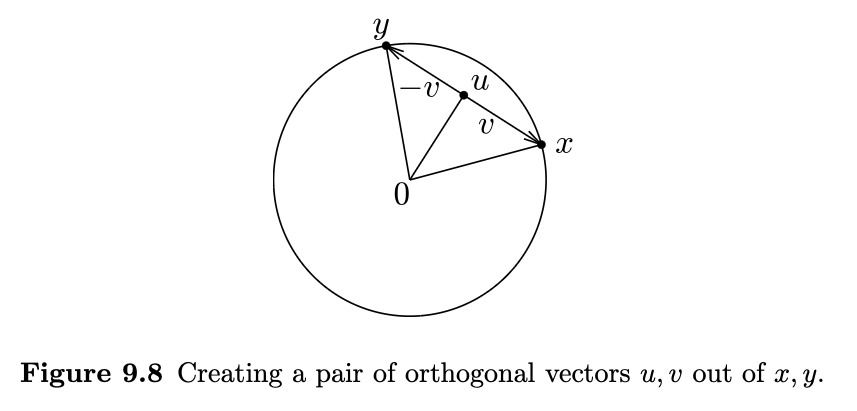
\includegraphics[width=0.8\textwidth]{Chapter 9/fig9-8.png}
\end{center}
Since $u, v$ are orthogonal, the Gaussian random vectors $Au$ and $Av$ are independent (Exercise 3.20).

\textbf{Step 2: Using Gaussian concentration.} Let's condition on $a := Au$ and study the conditional 
distribution of 
\[ f(Ax) = f(a + Av). \]
By independence, $a + Av$ is a Gaussian random vector that we can write as 
\[ a + Av = a + \lVert v \rVert_{2}g, \text{ where } g \sim N(0, I_m) \quad (\text{Exercise 3.20}) \]
We claim that the function 
\[ z \mapsto f(a + \lVert v \rVert_{2}z) \]
is Lipschitz with respect to the Euclidean norm on $\mathbb{R}^m$, with Lipschitz norm bounded by $\lVert v
\rVert_{2}$. To check this, fix any $t, s \in \mathbb{R}^m$ and use subadditivity of $f$ (in the form of 
Exercise 9.34) to get 
\begin{align*}
	f(a + \lVert v \rVert_{2}t) - f(a + \lVert v \rVert_{2}s) 
	&\leq f(\lVert v \rVert_{2}t - \lVert v \rVert_{2}s) \\
	&= \lVert v \rVert_{2} f(t - s) \quad \text{(Positive homogeneity)} \\
	&\leq \lVert v \rVert_{2} \lVert t - s \rVert_{2} \quad (b = 1),
\end{align*}
proving the claim.

Concentration in the Gauss space (\cref{thm:5.2.3}) then yields 
\[ \lVert f(a + Av) - \mathbb{E}_a\left[ f(a + Av) \right] \rVert_{\psi_2(a)}2 \leq C \lVert v \rVert_{2}, \]
where the index ``a" reminds us that these bounds are valid for the conditional distribution with $a = Au$ fixed.

\textbf{Step 3: Removing the conditioning.} Since the random vector $a - Av$ has the same distribution as that 
of $a + Av$, it satisfies the same bound:
\[ \lVert f(a - Av) - \mathbb{E}_a\left[ f(a - Av) \right] \rVert_{\psi_2(a)} \leq C \lVert v \rVert_{2}, \]
Subtract the bottom equation from the top one, use the triangle inequality and the fact that the expectations 
are the same gives 
\[ \lVert f(a + Av) - f(a - Av) \rVert_{\psi_2(a)} \leq 2 C \lVert v \rVert_{2}. \]
This bound holds conditionally for any fixed $a = Au$, Therefore, it holds for the original distribution too:
\[ \lVert f(a + Av) - f(a - Av) \rVert_{\psi_2} \leq 2 C \lVert v \rVert_{2}. \]
Passing back the the $x, y$ notation, we obtained the desired inequality.

We proved the theorem for unit vectors $x, y$. To extend it to the general case, argue exactly as step 4 in the 
proof of \cref{thm:9.1.2}.
\end{proof}

\begin{remark}[]
\label{rmk:9.6.5}
It is an open question if \cref{thm:9.6.3} holds for general subgaussian matrices $A$.
\end{remark}



% ----------9.7----------
\subsection{Two-sided Chevet Inequality and Dvoretzky-Milman Theorem}


\subsubsection{Two-sided Chevet's Inequality}
Another consequence of general matrix deviation is a sharper version of Chevet's inequality:

\begin{theorem}[Two-sided Chevet's inequality]
\label{thm:9.7.1}
Let $A$ be an $m \times n$ Gaussian random matrix with i.i.d $N(0, 1)$ entries. Let $T \subset \mathbb{R}^n$ and 
$S \subset \mathbb{R}^m$ be arbitrary bounded sets. Then 
\[ \mathbb{E}\left[ \sup_{x \in T} \left| \sup_{y \in S}\left\langle Ax, y \right\rangle - w(S) \lVert x 
\rVert_{2} \right| \right] \leq C \gamma(T) \mathrm{rad}(S), \]
where $\gamma(T)$ is the Gaussian complexity and $\mathrm{rad}(T)$ is the radius.
\end{theorem}

\begin{proof}
Let's apply \cref{thm:9.6.3} for the support function of $S$:
\[ f(x) = \sup_{y \in S}\left\langle x, y \right\rangle. \]
This is a bounded function, since the Cauchy-Schwartz inequality gives 
\[ f(x) \leq \sup_{y \in S}\lVert x \rVert_{2}\lVert y \rVert_{2} = \mathrm{rad}(S) \lVert x \rVert_{2} 
\text{ for all } x \in \mathbb{R}^n. \quad (*) \]
Since $Ax$ has the same distribution as $g \lVert x \rVert_{2}$ where $g \sim N(0, I_m)$ from Exercise 3.20, 
we have that 
\begin{align*}
	\mathbb{E}\left[ f(Ax) \right] 
	&= \lVert x \rVert_{2} \mathbb{E}\left[ f(g) \right] \quad (\text{Positive homogeneity}) \\
	&= \lVert x \rVert_{2} \mathbb{E}\left[ \sup_{y \in S}\left\langle x, y \right\rangle \right] \quad 
	\text{(By definition of )} f \\
	&= \lVert x \rVert_{2} w(S) \quad \text{(By definition of Gaussian width)}. \quad (**)
\end{align*}
Substitute $(*)$ and $(**)$ into \cref{thm:9.6.3} completes the proof.
\end{proof}


\subsubsection{Dvoretzky-Milman Theorem}
We'll now prove this amazing result: If you project any bounded set in $\mathbb{R}^n$ to a low-dimensional 
subspace, it will look \textit{approximately round} with high probability (Figure 9.9).

\begin{center}
	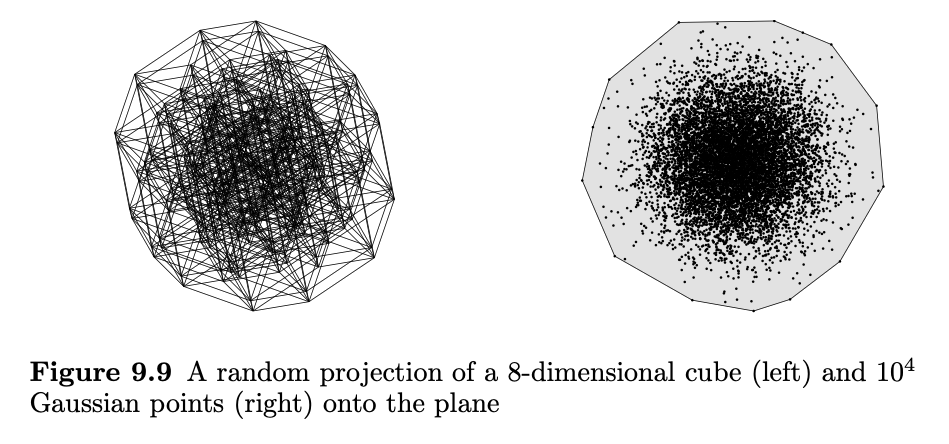
\includegraphics[width=0.8\textwidth]{Chapter 9/fig9-9.png}
\end{center}

It's easier to work with Gaussian projections, where the result says:
\begin{theorem}[Dvoretzky-Milman theorem]
\label{thm:9.7.2}
Let $A$ be an $m \times n$ Gaussian random matrix with i.i.d. $N(0, 1)$ entries, and $T \subset \mathbb{R}^n$ be 
a bounded subset. Then the following holds with probability at least 0.99:
\[ r_- B_2^m \subset \mathrm{conv}(AT) \subset r_+ B_2^m \]
where $B_2^m$ denotes the unit Euclidean ball in $\mathbb{R}^m$, and 
\[ r_{\pm} = w(T) \pm C \sqrt{m} \mathrm{rad}(T). \]
The left inclusion holds only if $r_-$ is nonnegative; the right inclusion always holds.
\end{theorem}

\begin{proof}
Let's use the two-sided Chevet's inequality (\cref{thm:9.7.1}) in the following form:
\[ \mathbb{E}\left[ \sup_{y \in S} \left| \sup_{x \in T}\left\langle Ax, y \right\rangle - w(T) \lVert y 
\rVert_{2} \right| \right] \leq C \gamma(S) \mathrm{rad}(T), \]
where $T \subset \mathbb{R}^n$ and $S \subset \mathbb{R}^m$. To get this, just apply the theorem to $A^T$ with 
$T$ and $S$ swapped.

Let $S$ be the sphere $S^{m - 1}$; its Gaussian complexity satisfies $\gamma(T) \leq \sqrt{m}$. Then, by 
Markov's inequality, the following holds with probability at least 0.99:
\[ \left| \sup_{x \in T}\left\langle Ax, y \right\rangle - w(T) \right| \leq C \sqrt{m} \mathrm{rad}(T) 
\text{ for every } y \in S^{m -1}. \]
By the triangle inequality and the definition of $r_{\pm}$, this implies 
\[ r_- \leq \sup_{x \in T}\left\langle Ax, y \right\rangle \leq r_+ \text{ for every } y \in S^{m - 1}. \]
Rewriting $\sup_{x \in T}\left\langle Ax, y \right\rangle$ as $\sup_{x \in AT}\left\langle x, y \right\rangle$ 
and using homogeneity, we get 
\[ r_- \lVert y \rVert_{2} \leq \sup_{x \in AT}\left\langle x, y \right\rangle \leq r_+ \text{ for every } 
y \in \mathbb{R}^m. \]
By duality (Exercise 9.40), this is the same as the statement of the theorem, and we're done!
\end{proof}

\begin{remark}[The effective dimension]
\label{rmk:9.7.3}
Assume that $T$ is bounded, convex, and contains the origin, and let 
\[ m \leq c d(T) \]
where $d(T) \asymp w(T)^2 / \mathrm{rad}(T)^2$ is the effective dimension (\cref{def:7.5.12}). If we pick the 
absolute constant $c$ to be small enough, we can make $C \sqrt{m} \mathrm{rad}(T) \leq 0.01 w(T)$, so that 
the Dvoretzky-Milman theorem (\cref{thm:9.7.2}) gives
\[ 0.99B \subset AT \subset 1.01B \]
with $B = w(T) B_2^n$ is the Euclidean ball of radius $w(T)$. In short: projecting \textit{any} bounded convex 
set $T$ onto a random subspace of dimension about $d(T)$ makes it look almost like a round ball!
\end{remark}

\begin{example}[Almost round projections of the cube]
\label{ex:9.7.4}
Consider the cube $T = [-1, 1]^n$. By \cref{ex:7.5.7}, 
\[ w(T) = \sqrt{2/\pi} \cdot n \text{ and } \mathrm{diam}(T) = 2 \sqrt{n} \]
So the effective dimension is $d(T) \asymp n$. So, if $m \leq cn$, then with high probability we have 
\[ 0.99B \subset A[-1, 1]^n \subset 1.01B \]
where $B$ is the Euclidean ball with radius $\sqrt{2/\pi} \cdot n$. In short: projecting an $n$-dimensional cube 
onto a subspace of dimension $m = cn$ makes it look almost like a round ball! Figure 9.9 gives an illustration.
\end{example}

\begin{remark}[Summary of random projections]
\label{rmk:9.7.5}
In sections 7.6 and 9.2.2, we found that a random projection $P$ of a set $T$ onto an $m$-dimensional subspace 
in $\mathbb{R}^n$ undergoes a phase transition. In the high-dimensional regime $(m \gtrsim d(T))$, the 
projection shrinks the diameter of $T$ by the factor of order $\sqrt{m/n}$: 
\[ \mathrm{diam}(PT) \asymp \sqrt{\frac{m}{n}} \mathrm{diam}(T)  \]
Moreover, the additive Johnson-Lindenstrauss lemma shows that in this regime, the random projection $P$ 
approximately preserves the geometry of $T$ (the distances between all points in $T$ shrink roughly by the same 
scaling factor).

In the low-dimensional regime $(m \lesssim d(T))$, shrinking stops:
\[ \mathrm{diam}(PT) \asymp w_s(T) \asymp \frac{w(T)}{\sqrt{n}} \]
regardless of how small $m$ is. The Dvoretzky-Milman theorem explains why: $PT$ is now an \textit{approximate 
round ball} of radius of order $w_s(T)$ (Exercise 9.43), which obviously does not shrink under any projection!
\end{remark}


